\section{Scattering}

The use of scattering techniques to probe soft condensed matter systems is commonplace. In this work, we have focussed on the use of small angle scattering (SAS), reflectometry, and grazing incidence small angle scattering (GiSAS) techniques. These are particularly appropriate for application to soft condensed matter systems due to the length scales capable of being probed being similar to the persistence length of the soft condensed matter systems. The length scales covered for such techniques is from around \SI{1}{\nano\metre} to \SI{100}{\nano\metre}, as is shown in Figure \ref{fig:lengths}. Since it is the equilibrium structures(s) under study, there is no interest in the system dynamics. Therefore, the system can be studied using exclusively elastic scattering techniques, where there is no energy transfer between the probing radiation and the system. This is in contrast to inelastic scattering where energy transfer occurs; facilitating the measurement of system dynamics, such as the dynamical modes of polymers of lipid bilayers.\cite{Sakai2009, Farago2009} The techniques mentioned above all involve the use of elastic scattering and therefore probe the system equilibrium structure.
%
\begin{figure}
	\centering
	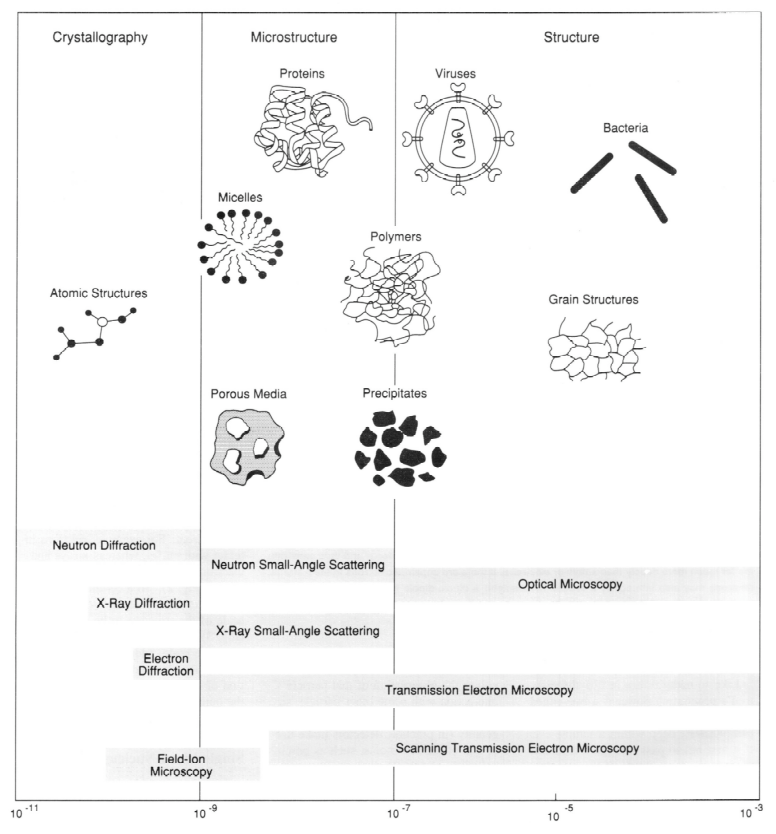
\includegraphics[width=0.7\textwidth]{theory/length}
	\caption{A representation of how different techniques can be used to probe various length scales, from Ref \cite{Sivia2011}.}
	\label{fig:lengths}
\end{figure}
%

Both X-ray and neutron scattering techniques are discussed and used in this work. From an experimental viewpoint, there are significant differences between an X-ray scattering and a neutron scattering experiment. However, there is little variation in terms of the data analysis, where the differences are limited to; the nature of the scattering lengths, and the higher background that is present in the neutron scattering experiments.

\subsection{The scattering vector}

The scattering of some probing radiation, by some sample can be represented as shown in Figure \ref{fig:scat}. Since only elastic scattering is being considered, there will be no change in the frequency of the radiation, $\omega_i = \omega_f$. This means that only the wavevector, $\mathbf{k}$, can change, $\mathbf{k}_i\neq \mathbf{k}_f$. The difference between the incident and final wavevectors is the scattering vector, $\mathbf{q}$, where,
%
\begin{equation}
	\mathbf{q} = \mathbf{k}_i - \mathbf{k}_f.
\end{equation}
%
%
\begin{figure}
	\centering
	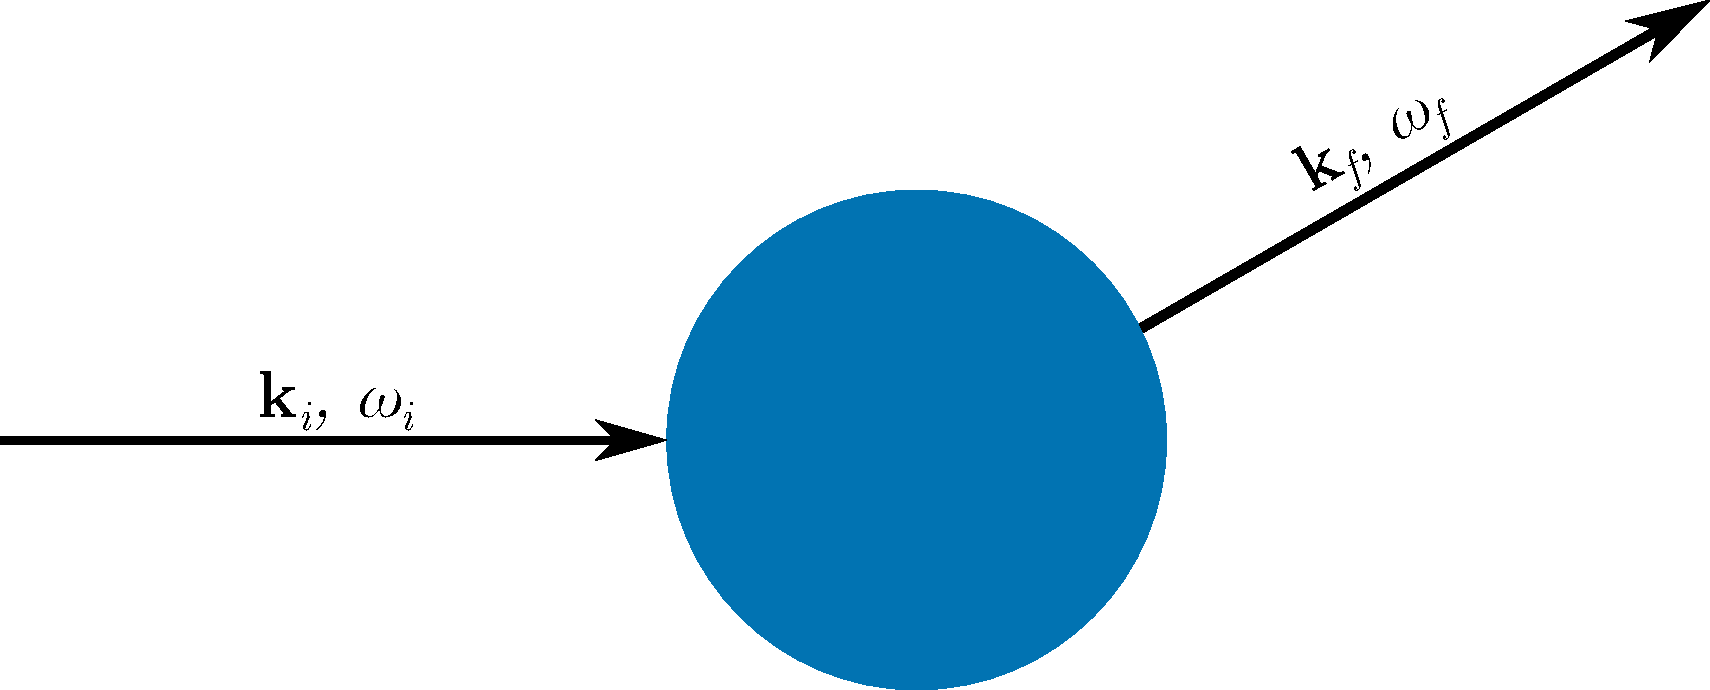
\includegraphics[width=0.7\textwidth]{theory/scat}
	\caption{A schematic of the scattering of some probing radiation by a sample (blue circle), adapted from Ref \cite{Sivia2011}.}
	\label{fig:scat}
\end{figure}
%
The scattering vector strictly has units of \si{\per\meter}, however it is often more practical to use \si{\per\nano\meter} or \si{\per\angstrom}. Throughout this work, units of reciprocal \AA ngstrom will be wherever possible. Since the frequency of the probing radiation does not change during an elastic scattering event, the wavelength, $\lambda$, will also not change, meaning that the moduli of the incident and final wavevectors are,
%
\begin{equation}
	|\mathbf{k}_i| = |\mathbf{k}_f|=\frac{2\pi}{\lambda}.
	\label{equ:wavevec}
\end{equation}
%
This means that only the angle will change during the elastic scattering event. The vector diagram in Figure \ref{fig:scatvec} can be used to describe the geometry of an elastic scattering event. From this, and Equation \ref{equ:wavevec}, the value of $q$, where $q = |\mathbf{q}|$ can be shown as,
%
\begin{equation}
	q = \frac{4\pi\sin{\theta}}{\lambda}.
	\label{equ:theq}
\end{equation}
%
\begin{figure}
	\centering
	
\includegraphics[width=0.7\textwidth]{theory/scatvec}
	\caption{A vector diagram describing an elastic scattering event, adapted from Ref \cite{Sivia2011}.}
	\label{fig:scatvec}
\end{figure}
%
However, this fails to fully capture the three dimensional nature of the scattering event. Hence, it is necessary to describe the scattering with spherical coordinates, $2\theta$, and $\phi$, such that the incoming and outgoing radiation can be described as,
%
\begin{equation}
	\begin{aligned}
		\mathbf{k}_i & = \bigg(0, 0, \frac{2\pi}{\lambda}\bigg), \\
		\mathbf{k}_f & = \frac{2\pi}{\lambda}(\sin{2\theta}\cos{\phi}, \sin{2\theta}\sin{\phi}, \cos{2\theta}),
	\end{aligned}
\end{equation}
%
where, $|\mathbf{k}_f| = \sfrac{2\pi}{\lambda}$. This allows the scattering vector to be written,
%
\begin{equation}
	\mathbf{q} = \frac{4\pi\sin{\theta}}{\lambda}(-\cos{\theta}\cos{\phi}, -\cos{\theta}\sin{\phi},\sin{\theta}).
\end{equation}
%
For an isotropic scattering pattern, it is the magnitude of the scattering vector, $q$, that is measured. In partical terms, the scattering vector allows for easy comparison of measurements made at different radiation wavelengths.

\subsection{Model-dependent analysis}

All types of scattering patterns can be analysed by one of two methods; model independent and model-dependent. The nature of this work means that it will focus on model-dependent analysis methods, often where the model is derived from some atomistic, or coarse-grained simulation. Model-dependent analysis, has significant benefits over model-independent methods, such as improved resoution and more detailed information of the structure. However, the necessisty of the inclusion of \emph{a priori} information within model-dependent analysis may act to bias the result, while this is undesirable, these assumptions can, and should, be educated based on the chemical information present -- such as the propensity for twin-tailed lipid molecules to for monolayers at an air-water interface.\cite{McCluskey2018}

The scattering from the model system is determined, using technique specific methods that are discuess in detail in laeter sections. This is then compared with the experimental data using some goodness-of-fit metric, as this the model is varied the quality of the fit, and therefore the value of the metric, will improve. In order to accurately reproduce the experimental measurement, it is necessary to include some instrumental resolution function, $res(q)$, in the modelling procedure. This is instrument specific, although it may be approximated by convolving the experimental dataset with some Gaussian smearing function, the modelled intensity can then be determined from,
%
\begin{equation}
	I(q) = res(q) * \frac{\text{d}\sigma(q)}{\text{d}\Omega},
\end{equation}
%
where, $\sfrac{\text{d}\sigma(q)}{\text{d}\Omega}$ is the differential cross-section, a measure of the number of scattering particles hitting a given solid angle of the detector.

The aim of model-dependent analysis is to obtain a model for the system which agrees will with the experimentally measured scattering data, while producing something that is chemically, and physically relevant. This means that optimisation algorithm are often applied to these analysis problems, which are discussed, in detail, in Section \ref{sec:optimisation}.

\subsection{Reflectometry}
Reflectometry involves the interaction of the probing radiation with some interface, from which the radiation is reflected. The geometry of a reflectometry experiment is shown in Figure \ref{fig:refgeo}, where the reflectometry instrument is in the horizontal configuration, ideal for the study of liquid interfaces. Reflectometry measurements give information about the structure perpendicular to the interface, the \emph{z}-dimension in Figure \ref{fig:refgeo}, and therefore the analysis of refllectometry data is founding on the assumption that the layers will be completely homogenous in the plane of the interface, the \emph{xy}-plane in Figure \ref{fig:refgeo}. In reality, since the layers are usually not completely homogeneous, an average is obtained for the area in the radiation beam.
%
\begin{figure}
	\centering
	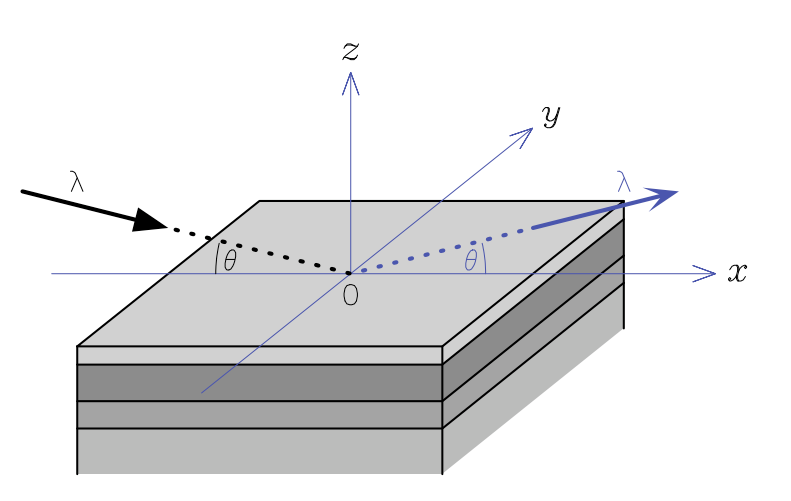
\includegraphics[width=0.7\textwidth]{theory/reflectgeo}
	\caption{A schematic of specular reflectometry from a layered sample, from Ref \cite{Sivia2011}.}
	\label{fig:refgeo}
\end{figure}
%
A reflectometry instrument operates by measuring the intensity of specular radiation at a series of different angles, $\theta$, or wavelengths, $\lambda$. The reflected intensity is defined in terms of $q$ (by Eqn \ref{equ:theq}), and is defined as follows,
%
\begin{equation}
	R(q) = \frac{\text{rate of specular reflective scattering}}{\text{rate of incidence}}.
	\label{equ:refl}
\end{equation}
%
It is clear from Equation \ref{equ:refl} that the value of the measured reflectometry cannot be greater than one, as this would mean that more particles of probing radiation were being reflected than were incident.

\subsubsection{Analysis}

There are two model-dependent analysis techniques that can be applied to the rationalisation of a reflectometry dataset. The first is the kinematic approach,\cite{Sivia2011} where the reflectometry profile is modelled in terms of the scattering length density profile in the \emph{z}-dimension, $\rho(z)$,
%
\begin{equation}
	R(q) \approx \frac{16\pi^2}{q^4}\bigg|\int_{-\infty}^{+\infty}\frac{\text{d}\rho(z)}{\text{d}z}\exp{(-izq)}\text{d}z\bigg|^2,
	\label{equ:kine}
\end{equation}
%
where, $\sfrac{\text{d}\rho(z)}{\text{d}z}$ is the first derivative of the scattering length density profile. However, this method has a significant problem, which can be described by applying Eqn \ref{equ:kine} to the scatteirng length density profile of a bare silicon substrate, which can be modelled as a Heaviside function (Figure \ref{fig:kine}a),
%
\begin{equation}
	\rho(z) =
  \begin{cases}
    0, & \text{if}\ z < 0 \\
    \rho_{\text{Si}}, & \text{otherwise}
  \end{cases}
\end{equation}
%
where, $\rho_{\text{Si}}$ is the scattering length denisty of pure silicon (\SI{2.1e-6}{\angstrom^{-2}} for neutrons). The derivated of a stepwise Heaviside function is a scaled $\delta$-function (Figure \ref{fig:kine}b),
%
\begin{equation}
	\rho'(z) = \rho_{\text{Si}}\delta(z).
\end{equation}
%
Then, as in Eqn \ref{equ:kine}, the Fourier transform of this $\delta$-function is taken,
%
\begin{equation}
	\rho_{\text{Si}}\int_{-\infty}^{+\infty}\delta(z)\exp{(-izq)}\text{d}z = \rho_{\text{Si}}\exp(0) = \rho_{\text{Si}}.
\end{equation}
%
This means that the reflectometry profile could be calculated from the following relationship,
%
\begin{equation}
	R(q)\approx \frac{16\pi^2\rho_{\text{Si}}^2}{q^4}.
\end{equation}
%
The curve from this relationship is shown in Figure \ref{fig:kine}, where it is clear that the agreement with an experimental profile would be poor as $q \rightarrow 0$. It can be seen that for low values of $q$ the calculated reflectometry is greater than 1, which voilates the physical constraint imposed with Eqn \ref{equ:refl}. This break down of the kinematic approach is due to the assumption present in this approach that the Born approximation will hold, that is that each particle of probing radiation will only be scattered once. However, in the reflectometry scattering geometry, this is no longer true rendering the kinematic approach invalid. 
%
\begin{figure}
	\centering
	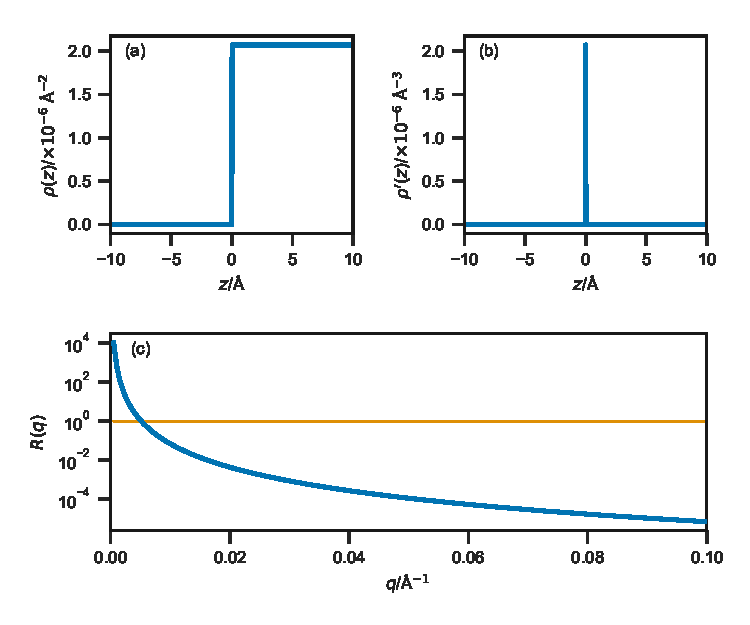
\includegraphics{theory/kine}
	\caption{A graphical representation of the kinematic approach; (a) the Heaviside function describing the scattering length density profile of a bare silicon substrate, (b) the $\delta$-function arising from the first derivative of the function in (a), and (c) the reflectometry profile resulting from Eqn \ref{equ:kine}, where the orange line at $R=1$ identifies the break down between experimental and theory in the kinematic approach, adapted from Ref \cite{Sivia2011}.}
	\label{fig:kine}
\end{figure}
%

\subsection{Small angle scattering}

\subsection{Grazing incidence small angle scattering}
